% !TeX root = ../../main.tex
\section{Hydraulic wash column design}\label{section: hydraulic wash column}

This section details the design of the hydraulic wash column, S106.

\subsection{Choice of wash column}   

 Initially, three types of wash column were considered: gravity, hydraulic, and mechanical. The main disadvantage with gravity wash columns is the long residence time, which can last as long as several hours, while hydraulic and mechanical wash columns have residence times of 10 to 15 minutes. Both hydraulic and mechanical wash columns are subject to compressive forces and pressure drops. Due to the use of moving mechanical parts in the mechanical wash column, it was considered a less desirable choice for this process. The hydraulic wash column was thus deemed the most suitable. This is a technique that combines continuous solid-liquid separation with counter-current washing. 

\subsection{Steady state model}   

Typically, the design of a hydraulic wash column should be based on pilot-scale experiments to determine appropriate dimensions at varying operating conditions. In this design, a model from van Oord-Knol \cite{van_oord-knol_hydraulic_2000} has been used for modelling the steady-state performance of the column. The hydraulic wash column has been modelled based on volume and force balances using initial dimensions provided by van Oord-Knol \cite{oordknol_dynamic_2002}. The aim of the modelling was to determine an appropriate steer flow rate, feasible column diameter, and the values of pressure at different sections of the wash column for attaining a 99.9 \% pure PNT product flow.  

% Typically, the design of a hydraulic wash column should be based on pilot-scale experiments to determine appropriate dimensions at varying operating conditions. In this design, a model from van Oord-Knol \cite{van_oord-knol_hydraulic_2000} has been used for modelling the steady-state performance of the column. The hydraulic wash column has been modelled based on volume and force balances using initial dimensions provided by van Oord-Knol \cite{oordknol_dynamic_2002}. Some variables were used to observe the performance of the column. The aim of this model was to determine an appropriate steer flow rate, feasible column diameter and determine the pressure at different sections of the wash column in  order to attain a 99.9 \% pure PNT product flow.  


\begin{wrapfigure}{r}{0.38\linewidth}
\centering
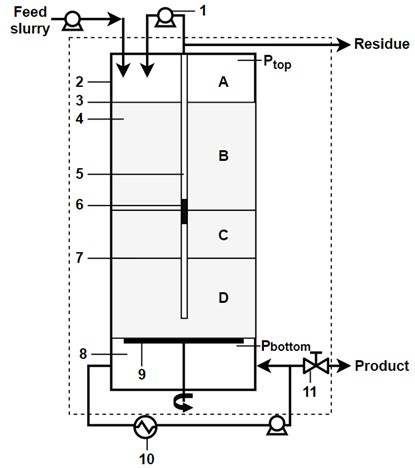
\includegraphics[width=0.35\textwidth]{chapters/3-separation/figures/hydraulic.jpg}
\caption{A schematic diagram of the hydraulic wash column: 1) steer flow pump 2) column wall 3) bed level 4) packed bed 5) filter tube 6) filter 7) wash front level 8) reslurry section 9) rotating knife 10) melter 11) product flow valve; A) slurry section B) filtration section C) stagnant section D) wash front section \cite{van_oord-knol_hydraulic_2000}}
\label{fig:hydraulic}
\end{wrapfigure}

\Cref{fig:hydraulic} illustrates the characteristics of the hydraulic wash column. The feed slurry is a mixture of the solid PNT crystals and the mother liquor consisting of MNT, the trace amount of ONT, and the remaining PNT that has not crystallised from the MSMPR crystalliser. The feed enters the column into the slurry section (2). Due to difference in density and hydraulic pressure, the solid crystals will fall down the column and sediment. The crystals form a moving packed bed of solid as they  move down the column. The filter tubes (6) remove the mother liquor from the filtration section. A part of the mother liquor gets recycled back into the column by the steer pump (1), known as the steer flow, and some mother liquor is purged out as residue or waste. The pressure drop across the filter drives the solids down the column and the mother liquor upwards through the filter tubes. This is where solid-liquid separation occurs. 

The densely packed moving bed in the wash front section contains a negligible amount of mother liquor. The rotating knife at the bottom scrapes the bottom of the packed bed, so that pure PNT solids fall into the bottom section. The melter melts the PNT solids and some of the molten solid gets pumped out as the product stream through the valve; some molten PNT ascends back into the bottom section and becomes the washing liquid, due to the pressure drop at the valve. The solid crystals, which are at a lower temperature, causes the washing liquid to crystallise on the solid particles, forming a frozen wash front level between the mother liquor and pure wash liquid. The wash liquid provides a counter current washing action where the displacement of mother liquor and washing of the liquid on the crystals results in pure crystals. TNO developed and demonstrated a hydraulic wash column with recovery greater than 99.9\% \cite{bassett_melt_2021}. The model has thus assumed 99.9 \% solid-liquid separation in the wash column with negligible amount of ONT and MNT impurity in the product flow and the wash front.

%A disadvantage of hydraulic wash column compared to gravity wash column  is that in gravity wash column some impurities are removed from the crystals via recrystallisation and sweating due to the long residence time in the column. Whereas, hydraulic wash columns have short residence time so the removal of the impurities trapped in crystal lattice is less likely to occur.   \cite{van_oord-knol_hydraulic_2000}.

\subsubsection{Volume balance} 
The model has been based on the assumption that the liquid and solid in the system are incompressible. Density and viscosity have been assumed to be independent of temperature. The overall volume balance at the top section is

\begin{equation}
\phi_{\mathrm{feed}}+\phi_{\mathrm{steer}}=\phi_{s,\mathrm{filters}}+\phi_{ml.\mathrm{filters}}
\end{equation}

\noindent where $\phi_{\mathrm{feed}}$ (m$^{3}$/s) is the feed flow, $\phi_{\mathrm{steer}}$ (m$^{3}$/s) is the steering flow, $\phi_{\mathrm{s,filters}} $(m$^{3}$/s) is the crystal flow at the filters and $\phi_{\mathrm{ml,filters}} $(m$^{3}$/s) is the mother liquor flow at the top section. The total length of the top section remains constant. The length of the filtration section $ L_{\mathrm{filtration}}$ (m), was derived from the solid balance in the top section: 

\begin{equation}
\frac{\dd L_{\mathrm{filtration}}}{\dd t} = \frac{1}{A_c(1-\alpha_2-\epsilon)}(\alpha_1\phi_{\mathrm{feed}}-\phi_{s,\mathrm{filters}})
\end{equation}

\noindent where $\alpha_1$ (m$^3$/m$^3$) is the crystal fraction in the feed slurry, $\alpha_2$ (m$^3$/m$^3$) is the crystal fraction in the slurry section, $\epsilon$ is the porosity in the filtration and stagnant section and $A_c $(m$^2$) is the cross sectional area of the wash column.

In the bottom section, there is the stagnant zone with the crystals. Then there is the wash zone with only the crystal and the wash liquid at steady state. The wash liquid crystallises due to low temperature at the wash front. The crystallisation of the wash liquid can be related to the disappearance of the wash liquid by difference in density of the solid and liquid.$C_s$ (m$^3$/s) is the solidification rate of wash liquid at the wash front, $C_l$ (m$^3$/s) is the washing liquid melted at the wash front. 
\begin{equation}
C_l= \frac{\rho_s}{\rho_l}C_s
\end{equation}

The amount of crystallised material was calculated based on a heat balance and temperature difference between the feed and the melt. This assumes the total cooling capacity of the crystals is used to crystallise the wash liquid:

\begin{equation}
C_s= \frac{c_p(T_{\mathrm{melt}}-T_{\mathrm{feed}})}{\Delta H_m}Q_{s,\mathrm{filters}}
\end{equation}

\noindent where $c_p$ (kJ kg$^{-1}$ K$^{-1}$) is the specific heat capacity, $T_{\mathrm{melt}} $(K) is the melting temperature, $T_{\mathrm{feed}}$ (K) is the feed temperature, and $\Delta H_m$ (kJ kg$^{-1}$) is the heat of fusion. 

The length of the wash section is related to the wash-liquid flow entering the knife and the wash liquid that crystallises. This assumes wash liquid is not lost through the filters which is ensured by positioning the filters above the wash section:

\begin{equation}
\epsilon_w A_c \frac{\dd L_{\mathrm{wash}}}{\dd t}= \phi_{wl,\mathrm{knife}}-C_l
\end{equation}

\noindent where $\epsilon_w$ is the porosity in the wash section, $L_{\mathrm{wash}}$ (m) is the length of the wash section and $\phi_{wl,\mathrm{knife}} $(\si{\cubic\m\per\s}) is wash liquid flow at the knife. 
The wash column during operation forms 3 layers of filtration, stagnant and wash sections. Within the filtration and stagnant sections, it is assumed that the porosity and permeability remain constant. Since the crystals form a densely packed column $\epsilon$ was approximated at 0.45 \cite{jansens_furification_1995}. Due to the wash-liquid crystallisation at the wash zone, an abrupt change in porosity and permeability was considered. The consolidation of the crystal bed were neglected in this model, however under compressive force from the pressure at the top section this may not be a valid assumption and will have to be explored further through experiments. The porosity in the wash zone was calculated from the equation below. 

\begin{equation}
\epsilon_{w}= \epsilon-(1-\epsilon)\left(\frac{c_p(T_{\mathrm{melt}}-T_{\mathrm{feed}})}{\Delta H_m}\right)
\end{equation}

At steady state, the wash section is constant with no flow of mother liquor into or out of the bottom section. The mother liquor at the top section leaves the column through the filter and splits into residual and steer flow. 

\begin{equation}
\phi_{\mathrm{residue}}= \phi_{ml,\mathrm{filters}} - \phi_{\mathrm{steer}}
\end{equation}

\noindent where $\phi_{\mathrm{residue}}$ (m$^3$/s) is the residue flow. 

The volume balance at the melting circuit is based on the assumption that crystals are molten the moment they enter the melting circuit. The wash liquid enters the column at the melting temperature.

\begin{equation}
\frac{\rho_s}{\rho_l}\phi_{s,\mathrm{knife}}= \phi_{wl,\mathrm{knife}} - \phi_{\mathrm{product}}
\end{equation}

\noindent where $\phi_{\mathrm{product}}$ (m$^3$/s) is the product flow.


\subsubsection{Force balance}
The liquid pressure drop across each section were calculated with the following modified Darcy's law equation. 

\begin{align}
    \frac{\Delta P_{l,\mathrm{filtration}}}{L_{\mathrm{filtration}}} &= \frac{\epsilon \eta_{l}}{B_{\mathrm{filtration}}}\left(\frac{\phi_{ml,\mathrm{filters}}}{\epsilon A_c} - \frac{\phi_{s,\mathrm{filters}}}{1-\epsilon A_c}\right) \\
    \frac{\Delta P_{l,\mathrm{stagnant}}}{L_{\mathrm{stagnant}}} &= \frac{\epsilon \eta_{l}}{B_{\mathrm{stagnant}}}\left(-\frac{\phi_{ml,\mathrm{bottom}}}{\epsilon A_c} - \frac{\phi_{s,\mathrm{filters}}}{1-\epsilon A_c}\right) \\
    \frac{\Delta P_{l,\mathrm{wash}}}{L_{\mathrm{wash}}} &= \frac{\epsilon \eta_{l}}{B_{\mathrm{wash}}}\left(-\frac{\phi_{wl,\mathrm{knife}}}{\epsilon_w A_c} - \frac{\phi_{s,\mathrm{knife}}}{1-\epsilon_w A_c}\right)
\end{align}

\noindent where $\Delta P_{l,\mathrm{filtration}}$, $\Delta P_{l,\mathrm{wash}}$, and $\Delta P_{l,\mathrm{stagnant}}$ (Pa) are the liquid pressure drops across the filtration, wash and stagnant section. $B_{\mathrm{filtration}},B_{\mathrm{wash}}$ and $B_{\mathrm{stagnant}}$ (m$^2$) are the permeability constants for filtration, wash and stagnant sections. The permeability constant at the filtration and stagnant section are equal. 

The permeability constants were determined  from Carman-Kozeny equation shown below. A commonly accepted value for Kozenzy constant, $K"$, is 5.

\begin{align}
   B_{\mathrm{filtration}} &= \frac{1}{K"}\frac{\epsilon^3}{S^2(1-\epsilon)^3} &
   B_{\mathrm{wash}} &= \frac{1}{K"}\frac{\epsilon_w^3}{S^2(1-\epsilon_w)^3}
\end{align}

The equation above is based on the assumption that the crystal particles are spherical so the specific surface area, $S$ (m$^2$), of particles is 

\begin{equation}
S = \frac{6}{d}
\end{equation}
\noindent where $d$ is the particle diameter. The liquid pressure gradient at each section were assumed to be constant since the packed bed is considered incompressible. The liquid pressure at the top in the slurry section was based on the pressure at the filter and the pressure drop over the filtration section. 
\begin{equation}
P_{\mathrm{top}} = P_{\mathrm{filters}} + \Delta P_{l,\mathrm{filtration}}
\end{equation}

\noindent whence $P_{\mathrm{top}}$ (Pa) is the liquid pressure above crystal bed and $P_{\mathrm{filters}} $(Pa) is the pressure at the filter. The pressure at the bottom is equal to the liquid pressure drop in the valve of the melting circuit, $\Delta P_{\mathrm{valve}} $(Pa). The pressure drop across the valve is determined through a linear relation with the product flow rate.
\begin{equation}
P_{\mathrm{bottom}}=\Delta P_{\mathrm{valve}} = K_w\phi_{\mathrm{product}}
\end{equation}
\noindent where $K_w$ (Pa~s/m$^3$) is the modified flow resistance factor. The pressure in the melting circuit was calculated using the equation below. 
\begin{equation}
\Delta P_{\mathrm{valve}} = \Delta P_{l,\mathrm{stagnant}} + \Delta P_{l,\mathrm{wash}} + P_{\mathrm{filters}}
\end{equation}

\subsection{Modelling results}
The linear system of algebraic equations from the steady state model were solved using input variables and parameters shown in \cref{tab:inputsparameters}. 

\begin{wraptable}{R}{0.53\linewidth}
\centering
\caption{Input variables and parameters}
\label{tab:inputsparameters}
\begin{tabular}{lS[table-format=1.2e2]s|lS[table-format=1.2e2]s}
\toprule
\multicolumn{3}{c|}{\textbf{Inputs}}                     & \multicolumn{3}{c}{\textbf{Parameters}}          \\ \midrule
$\phi_{\mathrm{feed}}$  & 4.27e5 & \cubic\m\per\s        & $\epsilon$                & 0.45     &           \\
$\phi_{\mathrm{steer}}$ & 2.65e5 & \cubic\m\per\s        & $\mathrm{B_{filtration}}$ & 1.37e-13 & \square\m \\
$\alpha_1$              & 0.906  & m$^3$/m$^3$                   & $\mathrm{B_{wash}}$       & 1.01e-13 & \square\m \\
$\mathrm{K_{w}}$        & 1.9e10 & \pascal\s\per\cubic\m &                           &          &           \\ \bottomrule
\end{tabular}
\end{wraptable}

During the operation of the hydraulic column, it is possible for the lengths of the filtration, stagnant, and wash sections to vary. With proper controls in place, the sections should not vary significantly to a normal mode of operation. Modelling with varying filtration and wash section lengths were implemented to observe their effect on pressures at different sections of the column. In the end, lengths of the filtration and wash sections have been designed to be between 0.27 to 0.30 m. 

\begin{figure}[h]
    \centering
    \begin{minipage}[t]{0.5\textwidth}
        \centering
        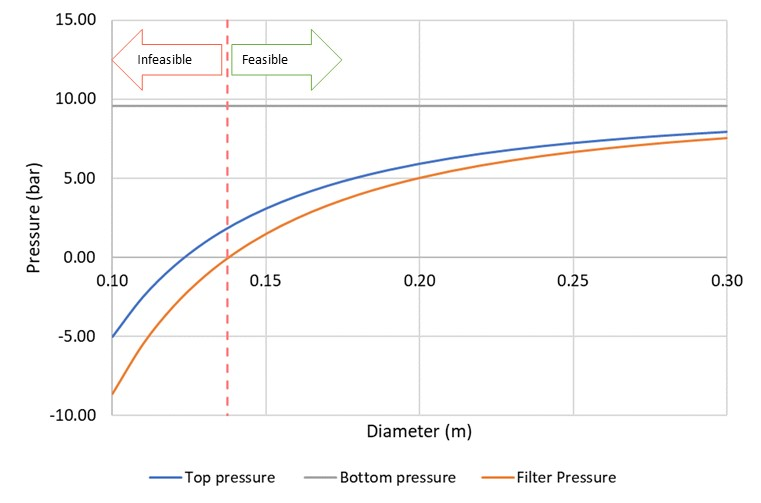
\includegraphics[width=\linewidth]{chapters/3-separation/figures/diameter.jpg}
        \caption{Effect of varying diameter on the pressure at top, bottom and filter section of the hydraulic wash column.} 
        \label{fig:dia_col}
        \end{minipage}%
    ~ 
    \begin{minipage}[t]{0.5\textwidth}
        \centering
        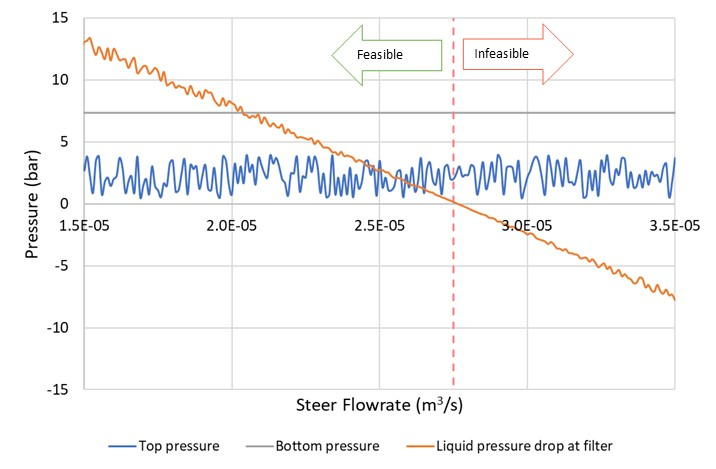
\includegraphics[width=\linewidth]{chapters/3-separation/figures/steerflow.jpg}
        \caption{Effect of varying steer flowrate on the pressure at top, bottom and filter section of the hydraulic wash column.}
    \label{fig:steer}   
    \end{minipage}

\end{figure}

Figures \ref{fig:dia_col} and \ref{fig:steer} show the effects of diameter and steer flowrate on the pressures in different sections of the column. The length of the column was designed to be 0.8 m. The diameter of the column was varied from 0.1 m to 0.3 m to observe the impact it has on the pressure across the column. Figure \ref{fig:dia_col} indicates when the diameter is less than 0.165 m, the model suggests negative pressure at the filter. This implies that instead of the mother liquor flowing upwards through the filter tube, it could be flowing in the reverse direction. The pressure at the top is also negative, which indicates that at these conditions the fluid flow in the column may not be in the desirable downward direction. A suitable diameter was chosen at 0.17 m allowing for slight variations in the section lengths over time under normal operation.

Steer flow is the flow rate of the mother liquor being recycled back into the column from the filter tubes while some mother liquor is removed as residual flow. The filtrate that is recycled back into the column increases the transport force. The steer flowrate was varied from $1.5 \times 10^{-5}$ to $3.5 \times 10^{-5}$ $m^{3}/s$. Figure \ref{fig:steer} shows the infeasible and feasible regions of operation. Above a steer flow rate of $2.7 \times 10^{-5}$ $m^{3}/s$, the model indicates a negative liquid pressure drop at the filter. However, at lower steer flows such as $1.5 \times 10^{-5}$ $m^{3}/s$, the filter pressure increases significantly to more than 10 bar. In order to attain a lower pressure but also to ensure that the column is operating in a feasible region, the steer flow rate at $2.65 \times 10^{-5}$ $m^{3}/s$ was chosen. At this flow rate, there is an allowance for variations in the flowrate whilst still allowing the column to operate in the feasible region. The steer flow appears to have no impact on the bottom pressure. This is because the bottom pressure mainly relies on the valve resistance coefficient. 

\begin{wrapfigure}{R}{0.5\linewidth}
\centering
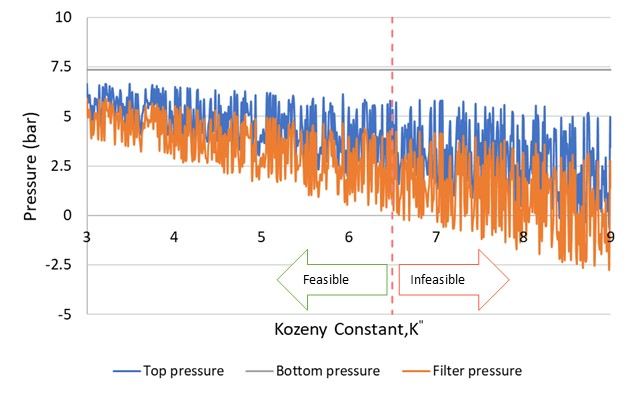
\includegraphics[width=\linewidth]{chapters/3-separation/figures/kozeny.jpg}
\caption{Effect of varying Kozeny constant on  on the pressure at top, bottom and filter section of the hydraulic wash column.}
\label{fig:koz_col}
\end{wrapfigure}

The permeability constant, $B$, was determined using the Kozeny constant, $K"$.  In this process, $K"$ was considered to be 5, assuming the crystal is spherical. A sensitivity analysis on the permeability constant was conducted by varying K". \Cref{fig:koz_col} shows that when $K"$ > 6.5, the design becomes infeasible as negative filter pressures are reached. The sensitivity analysis was conducted with the filtration and wash section varying between 0.27 and 0.3 m to observe the range of pressures in the column. It is evident that the hydraulic column is sensitive to the Kozenzy constant and the permeability of the packed bed. This was expected due to the inverse relationship between the permeability constant and pressure drop in the modified Darcy's law equation. Thus, it is essential to conduct pilot-scale experiments to obtain more accurate values for K" and the permeability constant to get a reliable observation of the column's performance. 

The pressure of the top, bottom, and filter sections are 4.02 bar, 2.79 bar, 7.36 bar respectively. Based on literature \cite{jansens_furification_1995} the temperature profile at the wash front was found to be independent of the axial and radial position in the column if the distance of the wash front from the filter is greater than 0.1 m. The temperature profile was also found to be independent of the product throughput. Additionally, compressive stress impacts the permeability of the bed and causes deformation of the crystal particles. In this process the crystals are melted; the crystal particle size or shape were not of concern so compressive stress was not considered further. 

%In this design the filter tube was positioned 0.1 m above the wash front. 

Table \ref{tab:wash column stream table} is a stream table for the hydraulic wash column. For the melter, H301, at the bottom, a 3.69 kW heating duty is required.  

\begin{table}[h]
\centering
\caption{Stream table for the hydraulic wash column.}
\label{tab:wash column stream table}
\begin{tabular}{@{}l|l|l|l|l|l|l|l|l|l@{}}
\toprule
Stream            & 3-01 & 3-02 & 3-03 & 3-04 & 3-05 & 3-06 & 3-07 & 3-08 & 3-09 \\ \midrule
Temperature (K)   & 280 & 324 & 324 & 324 & 324 & 280 & 280 & 280 & 324 \\ \midrule
Pressure (bar)    &  4.02  & 7.36   & 7.36   & 7.36   & 7.36   & 2.79   & 4.02   & 2.79   & 1.01 \\ \midrule
Phase & \begin{tabular}[c]{@{}l@{}}Solid \\ + liquid \end{tabular}  & \begin{tabular}[c]{@{}l@{}}Solid \\ + liquid \end{tabular} & Liquid & Liquid & Liquid & Liquid & Liquid & Liquid & Liquid \\ \midrule
Liquid fraction &  0.1995 &  0.1995 & 1 & 1 & 1 & 1 & 1 & 1 & 1\\ \midrule
Solid fraction  &  0.8005  &  0.8005 & 0 & 0 & 0 & 0 & 0 & 0 & 0 \\ \midrule
MNT (kmol/day)  &  2.72 & 0.00 & 0.00 & 0.00 & 0.00 & 10.55 & 10.55 & 2.72 & 0.00 \\ \midrule
ONT (kmol/day)  &  0.17 & 0.00 & 0.00 & 0.00 & 0.00 & 0.67 & 0.67 & 0.17 & 0.00 \\ \midrule
PNT (kmol/day)  &  21.99 & 22.48 & 22.48 & 2.58 & 19.90 & 8.12 & 8.12 & 2.09 & 19.90\\ \bottomrule
\end{tabular}
\end{table}

\subsection{Physical design}

\begin{wraptable}{R}{0.4\linewidth}
\centering
\caption{Summary of key physical design parameters for the hydraulic wash column.}
\label{tab:wash column mech design summary}
\begin{tabular}{@{}l|l@{}}
\toprule
\textbf{Inner diameter (mm)}                &    170.00 \\ \midrule
\textbf{Height of cylindrical shell (mm)}   & 800.00 \\ \midrule
\textbf{Crown radius (mm)}                  & 136.00 \\ \midrule
\textbf{Knuckle radius (mm)}                & 24.82  \\ \midrule
\textbf{NPS of sightholes (inch)}                & 2 \\ \midrule
\textbf{NPS of all other ports (inch)}                & 1/2 \\ \midrule
\textbf{Flange class}                       & 300 \\ \midrule
\textbf{Knife length (mm)}              & 156.00 \\ \midrule
\textbf{Number of knives}            & 4 \\ \midrule
\textbf{Knife width (mm)}          & 6.5 \\ \bottomrule
\end{tabular}
\end{wraptable}
The hydraulic wash column vessel has also been designed in accordance with British Standards and to consist of a cylindrical shell and two ellipsoidal domed ends. From \textbf{BS5500: 1997}, the minimum thickness for a cylindrical shell, $e_{\mathrm{cyl}}$, can be computed as 

\begin{equation}
    e_{\mathrm{cyl}} = \frac{P D_i}{2f - P}
\end{equation}

\noindent where $P$ is the highest design pressure in the vessel which is 7.36 bar and $D_i$ is the internal diameter of the vessel taken to be the same as $D$ as defined in \cref{sec: crystalliser mass balance}. For a vessel with ellipsoidal ends, the minimum thickness, $e_{\mathrm{end}}$, can be calculated using the methodology outlined in Section 3.5.2 of \textbf{BS5500: 1997}. The values of $e_{\mathrm{cyl}}$ and $e_{\mathrm{end}}$ have been obtained as 0.36 mm and 0.918 mm. After a corrosion factor of 1.5 mm has been taken into account, a uniform wall thickness of 3 mm has been chosen for both the shell and the dome ends. 

Eight ports are required in total: the inlet, the top recycle, the filter tube outlet, the outlet, the bottom recycle, a safety relief valve, and two sightholes. The safety relief valve is able to release the liquid level in the vessel to 80\% from maximum-allowable working pressure (MAWP) designed to be 1.21 times $P$ in less than 1 min. Schedule 80 pipes with nominal pipe size (NPS) of 1/2 inch have been selected for all ports except the two sightholes on the wash column. For the two sightholes, 2 inch pipes have been used instead. 

Four filter tubes 680 mm in length, 20 mm in diameter, and 3 mm in wall thickness have been implemented in the design. A set of four knives have been implemented at the bottom of the vessel. Support structures are not included in the design but are nonetheless recommended for implementation due to the inherent imbalance of weights. 

Schematics and GA drawing for the design is available in Figures \ref{fig:wash column GA} and \ref{fig:wash column schematic}. Table \ref{tab:wash column mech design summary} gives a summary of the physical design. 

